\documentclass[11pt,fullpage]{article}
\usepackage{color, soul}
\usepackage{multicol,amsmath,amssymb,algorithmic}
\usepackage{graphics,graphicx}
\usepackage[right = 2.5cm, left=2.5cm, top = 2.5cm, bottom =2.5cm]{geometry}
\usepackage{enumerate}
\usepackage{bm}
\usepackage[colorlinks,linkcolor=blue,anchorcolor=blue,citecolor=blue]{hyperref}
\pagestyle{plain}
\def\urlfont{\DeclareFontFamily{OT1}{cmtt}{\hyphenchar\font='057}
              \normalfont\ttfamily \hyphenpenalty=10000}

%\input macros

\newcommand{\subheading}[1]{\noindent \textbf{#1}}
\newcommand{\grad}{\nabla}
\newcommand{\jump}[1]{[#1]}
\newcommand{\limit}[2]{\lim_{#1 \rightarrow #2}}
\newcommand{\mb}[1]{\mathbf{#1}}
\newcommand{\reals}[1]{\mathbb{R}^{#1}}
%\newcommand{\blue}[1]{{\color{blue}{{#1}}}}
\newcommand{\blue}[1]{#1}

\title{Peridynamics-Based Fracture Animation for Elastoplastic Solids:\\
      Supplementary Technical Document}

\begin{document}
\maketitle

\section{Introduction}

This document presents the derivation of the constitutive model proposed in the paper. Section \blue{\ref{section:2}} introduces some preliminaries for the derivation and explains why the classical continuum elasticity theory could be regarded as a special case of peridynamics. Section \blue{\ref{section:3}} lists the common procedures to derive the peridynamics formulation of a general hyperelastic constitutive model in continuum mechanics. Finally, section \blue{\ref{section:4}} presents the derivation of the model introduced in the paper, which is a \emph{nonlocal} extension of the linear elastic model in the \emph{local} theory.

\section{Preliminaries}\label{section:2}

\subsection{Peridynamics equations of motion and the discretization}

As is introduced in the paper, the peridynamics governing equation for any material point located at $\mb{x}$ is formulated as below:
\begin{equation}
\rho\ddot{\mb{u}}(\mb{x}) = \int_{H_\mb{x}}[\mb{T}\langle\mb{x}',\mb{x}\rangle - \mb{T}\langle\mb{x},\mb{x}'\rangle]dV_{\mb{x}'}+\mb{b}(\mb{x}).
\label{eq:1}
\end{equation}
The state of material point at $\mb{x}$ is influenced by the possibly infinite number of material points $\mb{x}'$ that belong to its family $H_\mb{x}$. When the continuum is discretized into particles, the integral in Equation \blue{\ref{eq:1}} is replaced with the summations of particles within the horizon $\delta_\mb{x}$:
\begin{equation}
\rho\ddot{\mb{u}}(\mb{x}) = \sum_{\mb{x}',\mb{x}'\in H_\mb{x}}[\mb{T}\langle\mb{x}',\mb{x}\rangle - \mb{T}\langle\mb{x},\mb{x}'\rangle]V_{\mb{x}'}+\mb{b}(\mb{x}),
\label{eq:2}
\end{equation}
where $V_{\mb{x}'}$ is the volume of the discrete particle and its value depends on the distribution of particles.
\subsection{Peridynamics for local interactions}

In the limiting case where the horizon $\delta_\mb{x}$ approaches 0, the material point $\mb{x}$ interacts only with its immediate neighbors. See Figure \blue{\ref{fig:1}}, the material point with label $k$ interacts with the other six material points in the immediate vicinity denoted as $(k-l)$,$(k+l)$,$(k-m)$,$(k+m)$,$(k-n)$,and $(k+n)$. This conforms to the classical continuum mechanics, see the book \blue{\cite{bonet2008nonlinear}} for reference.
\begin{figure}[h]
  \centering
  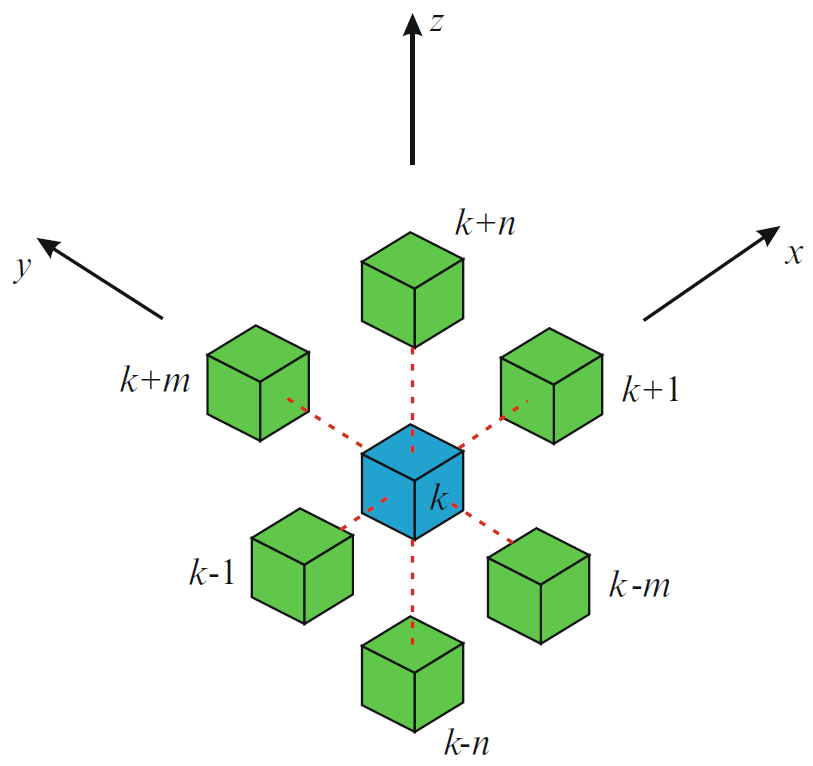
\includegraphics[width=0.5\linewidth]{./fig1.png}
  \caption{\label{fig:1}
  Material point $k$ interacts with its immediate neighborhood. Image from \blue{\cite{madenci2014peridynamic}}.
}
\end{figure}

In the context of local interactions, Equation \blue{\ref{eq:2}} for material point $k$ is represented in the following form:
\begin{equation}
\rho_{(k)}\ddot{\mb{u}}_{(k)} = \sum_{j=k-l,k+l,k-m,k+m,k-n,k+n}(\mb{t}_{(k)(j)}-\mb{t}_{(j)(k)})V_{(j)} + \mb{b}_{(k)},
\label{eq:3}
\end{equation}
where $\mb{t}_{(k)(j)}$ denotes the internal force density that material point $j$ exerted on point $k$, and $\mb{t}_{(j)(k)}$ is the other way around.

Let's recall the form of governing equations in continuum mechanics:
\begin{equation}
\rho_{(k)}\ddot{\mb{u}}_{(k)} = \nabla\cdot\sigma_{(k)} + \mb{b}_{(k)},
\label{eq:4}
\end{equation}
where $\sigma_{(k)}$ is the cauchy stress at point $k$. We could further write it in a component-wise form and approximate the spatial derivatives with central difference. Take the $x$-component as an example:
\begin{equation}
\begin{aligned}
\rho_{(k)}\ddot{\mb{u}}_{x(k)} &= \quad \frac{1}{2}\frac{\sigma_{xx(k)} - \sigma_{xx(k-l)}}{\Delta x} + \frac{1}{2}\frac{\sigma_{xx(k+l)} - \sigma_{xx(k)}}{\Delta x}\\
                              &\quad+  \frac{1}{2}\frac{\sigma_{xy(k)} - \sigma_{xy(k-m)}}{\Delta y} + \frac{1}{2}\frac{\sigma_{xy(k+m)} - \sigma_{xy(k)}}{\Delta y}\\
                              &\quad+  \frac{1}{2}\frac{\sigma_{zx(k)} - \sigma_{zx(k-n)}}{\Delta z} + \frac{1}{2}\frac{\sigma_{xz(k+n)} - \sigma_{xz(k)}}{\Delta z}\\
                              &\quad + \mb{b}_{x(k)}.
\end{aligned}
\label{eq:5}
\end{equation}
Each term in the above equation involves only material point $k$ and one immediate neighbor. We could recast Equation \blue{\ref{eq:3}} in a similar form:
\begin{equation}
\begin{aligned}
\rho_{(k)}\ddot{\mb{u}}_{(k)} &= \quad (\mb{t}_{(k)(k-l)} - \mb{t}_{(k-l)(k)})V_{(k-l)} + (\mb{t}_{(k)(k+l)} - \mb{t}_{(k+l)(k)})V_{(k+l)}\\
                             &\quad + (\mb{t}_{(k)(k-m)} - \mb{t}_{(k-m)(k)})V_{(k-m)} + (\mb{t}_{(k)(k+m)} - \mb{t}_{(k+m)(k)})V_{(k+m)}\\
                             &\quad + (\mb{t}_{(k)(k-n)} - \mb{t}_{(k-n)(k)})V_{(k-n)} + (\mb{t}_{(k)(k+n)} - \mb{t}_{(k+n)(k)})V_{(k+n)}\\
                             &\quad  + \mb{b}_{(k)}.
\end{aligned}
\label{eq:6}
\end{equation}
By equating Equation \blue{\ref{eq:5}} (and its counterparts) with Equation \blue{\ref{eq:6}}, we get the relationships between the cauchy stress and the peridynamics internal force density:
\begin{equation}
\sigma_{\alpha\beta(k)} = 2t_{\beta(k)(q_\alpha)}\Delta\alpha V_{(q_\alpha)}\qquad \mathrm{with } \quad q_x=(k+l),q_y=(k+m),q_z=(k+n)
\label{eq:7}
\end{equation}
\begin{equation}
\sigma_{\alpha\beta(k)} = -2t_{\beta(k)(q_\alpha)}\Delta\alpha V_{(q_\alpha)}\qquad \mathrm{with } \quad q_x=(k-l),q_y=(k-m),q_z=(k-n),
\label{eq:8}
\end{equation}
where $\alpha,\beta=x,y,z$. Especially, for normal stress, we would have:
\begin{equation}
\sigma_{\alpha\alpha} = 2 \mb{t}_{(k)(q_\alpha)}\cdot(\mb{x}_{(q_\alpha)}-\mb{x}_{k})V_{(q_\alpha)}.
\label{eq:9}
\end{equation}
The subsequent equation would also be useful for the derivation in following sections:
\begin{equation}
\begin{aligned}
\sum_{\beta=x,y,z}\sigma_{\alpha\beta(k)}^2 &= \sum_{\beta=x,y,z}4t_{\beta(k)(q_\alpha)}^2(\Delta\alpha)^2 V_{(q_\alpha)}^2 \\
                                            &= 4(\mb{t}_{(k)(q_\alpha)}|\mb{x}_{(q_\alpha)}-\mb{x}_{k}|V_{(q_\alpha)})
                                                 \cdot
                                                (\mb{t}_{(k)(q_\alpha)}|\mb{x}_{(q_\alpha)}-\mb{x}_{k}|V_{(q_\alpha)}).
\end{aligned}
\label{eq:10}
\end{equation}

\subsection{Strain energy density and internal force density}

In continuum mechanics the hyperelastic constitutive models are generally represented as strain energy densities. Therefore it is necessary to define the relationship between strain energy density and peridynamics internal force density. According to the book by Madenci and Oterkus\blue{\cite{madenci2014peridynamic}}, in ordinary state-based peridynamics the relationship is defined as below:
\begin{equation}
\mb{t}_{(k)(j)}=\frac{1}{V_{(j)}}\frac{\partial W_{(k)}}{\partial (|\mb{y}_{(j)}-\mb{y}_{(k)}|)}\frac{\mb{y}_{(j)}-\mb{y}_{(k)}}{|\mb{y}_{(j)}-\mb{y}_{(k)}|},
\label{eq:11}
\end{equation}
in which $W_{(k)}$ is the strain energy density at material point $k$. The force density vector is aligned with the relative position vector in the deformed configuration and it can be defined in the form
\begin{equation}
\mb{t}_{(k)(j)} = \frac{1}{2}A\frac{\mb{y}_{(j)}-\mb{y}_{(k)}}{|\mb{y}_{(j)}-\mb{y}_{(k)|}}
\label{eq:12}
\end{equation}
and
\begin{equation}
\mb{t}_{(j)(k)} = -\frac{1}{2}B\frac{\mb{y}_{(j)}-\mb{y}_{(k)}}{|\mb{y}_{(j)}-\mb{y}_{(k)|}},
\label{eq:13}
\end{equation}
where $A$ and $B$ are auxiliary parameters that are dependent on engineering material constants, deformation field, and the horizon.


\section{Derivation for general hyperelastic materials}\label{section:3}

Given the strain energy representation of a general hyperelastic material in continuum mechanics, we could obtain the explicit form of its peridynamics internal force density following some common procedures. Once we get the explicit form of the force density, we could further derive the peridynamics version of governing equations and proceed with the simulation.

The derivation procedures for a general hyperelastic material are listed below:
\begin{enumerate}
\item{Represent the strain energy density $W$ in terms of the internal force density $\mb{t}$, using the relationships in Equation \blue{\ref{eq:7}} \~{} \blue{\ref{eq:10}}. The strain energy densities in continuum mechanics are generally represented in terms of the stress tensor $\sigma$, or could be easily recast into this form. Then the derivation to the peridynamics form is straightforward with the relationships between $\sigma$ and $\mb{t}$.}
\item{Substitute the form of $\mb{t}$ (Equation \blue{\ref{eq:12}} and \blue{\ref{eq:13}}) into the representation of $W$ and perform differentiation using Equation \blue{\ref{eq:11}}. The resulting explicit expression of $\mb{t}$ contains several auxiliary parameters.}
\item{Determine the material parameters by equating the strain energy representations in continuum mechanics with their counterparts in peridynamics under several simple loading cases. The loading cases are carefully chosen so that the strain energy density could be analytically computed with the continuum mechanics representation. Then by equating the energy value with the peridynamics form of strain energy density, we could determine the peridynamics material parameters.}
\end{enumerate}

\section{Derivation for linear elastic materials}\label{section:4}

We choose to design our peridynamics constitutive model based on the linear elastic model in continuum mechanics due to its simplicity. More general hyperelastic models could be derived following the same procedures introduced above. For instance, Bang\blue{\cite{bang2016peridynamic}} performed derivations for the incompressible Neo-Hookean material.

\subsection{Strain energy density in terms of force density}

For an isotropic linear elastic material, the explicit form of the strain energy density, $W_{(k)}$, at material point $k$ can be represented as:
\begin{equation}
W_{(k)} = \frac{\kappa}{2}\theta_{(k)}^2+\left[\frac{1}{4\mu}(\sigma_{xx(k)}^2+\sigma_{yy(k)}^2+\sigma_{zz(k)}^2)
                                         +\frac{1}{2\mu}(\sigma_{xy(k)}^2+\sigma_{xz(k)}^2+\sigma_{yz(k)}^2)
                                         -\frac{3\kappa^2}{4\mu}\theta_{(k)}^2
                                    \right],
\label{eq:14}
\end{equation}
in which $k$ and $\mu$ are the bulk modulus and the shear modulus. Note that we ignore the temperature change in the course of deformation. The first term and the second term at the right-hand side of the equation represent the dilatational energy and the distortional energy, respectively. The dilatation, $\theta_{(k)}$ is defined through
\begin{equation}
\theta_{(k)} = \epsilon_{xx(k)}+\epsilon_{yy(k)}+\epsilon_{zz(k)} = \frac{\sigma_{xx(k)}+\sigma_{yy(k)}+\sigma_{zz(k)}}{3\kappa}.
\label{eq:15}
\end{equation}
We rearrange the strain energy density to a slightly different form:
\begin{equation}
\begin{aligned}
W_{(k)} =& \frac{\kappa}{2}\theta_{(k)}^2 -\frac{3\kappa^2}{4\mu}\theta_{(k)}^2 \\
         &+\frac{1}{8\mu}\left[(\sigma_{xx(k)}^2+\sigma_{xy(k)}^2+\sigma_{xz(k)}^2) + (\sigma_{xx(k)}^2+\sigma_{xy(k)}^2+\sigma_{xz(k)}^2)\right]\\
         &+\frac{1}{8\mu}\left[(\sigma_{yx(k)}^2+\sigma_{yy(k)}^2+\sigma_{yz(k)}^2) + (\sigma_{yx(k)}^2+\sigma_{yy(k)}^2+\sigma_{yz(k)}^2)\right]\\
         &+\frac{1}{8\mu}\left[(\sigma_{zx(k)}^2+\sigma_{zy(k)}^2+\sigma_{zz(k)}^2) + (\sigma_{zx(k)}^2+\sigma_{zy(k)}^2+\sigma_{zz(k)}^2)\right],
\end{aligned}
\label{eq:16}
\end{equation}
where each term involves stress component corresponds to the contribution from one of its immediate neighborhood $(k-l)$,$(k+l)$,$(k-m)$,$(k+m)$,$(k-n)$ and $(k+n)$.
Utilizing the relationship by Equation \blue{\ref{eq:10}} leads to the following result:
\begin{equation}
\begin{aligned}
W_{(k)} =& (\frac{\kappa}{2} -\frac{3\kappa^2}{4\mu})\theta_{(k)}^2 \\
         &+\frac{1}{2\mu}\sum_{\substack {j=k-l,k+l,\\ \quad k-m,k+m,\\ \quad k-n,k+n}}(\mb{t}_{(k)(j)}|\mb{x}_{(j)}-\mb{x}_{(k)}|V_{(j)})\cdot(\mb{t}_{(k)(j)}|\mb{x}_{(j)}-\mb{x}_{(k)}|V_{(j)}).
\end{aligned}
\label{eq:17}
\end{equation}

We can also rewrite the dilatation, $\theta_{(k)}$, in a slightly different form as:
\begin{equation}
\begin{aligned}
\theta_{(k)} =& \frac{\sigma_{xx(k)}+\sigma_{yy(k)}+\sigma_{zz(k)}}{3\kappa}\\
        =& \frac{1}{3\kappa}(\frac{1}{2}\sigma_{xx(k)}+\frac{1}{2}\sigma_{yy(k)}+\frac{1}{2}\sigma_{zz(k)}
         + \frac{1}{2}\sigma_{xx(k)}+\frac{1}{2}\sigma_{yy(k)}+\frac{1}{2}\sigma_{zz(k)}).
\end{aligned}
\label{eq:18}
\end{equation}
Substitute Equation \blue{\ref{eq:9}} into the above equation, we get the explicit form of $\theta_{(k)}$ in terms of $\mb{t}_{(k)}$:
\begin{equation}
\theta_{(k)} = \frac{1}{3\kappa}\left(\sum_{\substack {j=k-l,k+l,\\ \quad k-m,k+m,\\ \quad k-n,k+n}}(\mb{t}_{(k)(j)}\cdot(\mb{x}_{(j)}-\mb{x}_{(k)})V_{(j)})\right).
\label{eq:19}
\end{equation}

Combining Equation \blue{\ref{eq:17}} and Equation \blue{\ref{eq:19}} leads to the representation of strain energy density $W_{(k)}$ in terms of internal force density $\mb{t}_{(k)(j)}$.

\subsection{Explicit form of force density}

For isotropic linear elastic materials, the internal force between material points is linear in magnitude with respect to the stretch of the bond between them. Therefore, the internal force density $\mb{t}_{(k)(j)}$ could be written in a more specific form:
\begin{equation}
\mb{t}_{(k)(j)} = \frac{1}{2}cs_{(k)(j)}\frac{\mb{y}_{(j)} - \mb{y}_{(k)}}{|\mb{y}_{(j)} - \mb{y}_{(k)}|},
\label{eq:20}
\end{equation}
with
\begin{equation}
s_{(k)(j)} = \frac{|\mb{y}_{(j)} - \mb{y}_{(k)}| - |\mb{x}_{(j)} - \mb{x}_{(k)}|}{|\mb{x}_{(j)} - \mb{x}_{(k)}|}
\label{eq:21}
\end{equation}
being the stretch between two material points. $c$ amounts to constant elastic coefficient of spring forces.

Substituting Equation \blue{\ref{eq:20}} into Equation \blue{\ref{eq:17}} and \blue{\ref{eq:19}} results in:
\begin{equation}
\begin{aligned}
W_{(k)} =& (\frac{\kappa}{2} -\frac{3\kappa^2}{4\mu})\theta_{(k)}^2 \\
         &+\frac{c^2}{8\mu}\sum_{\substack {j=k-l,k+l,\\ \quad k-m,k+m,\\ \quad k-n,k+n}}(s_{(k)(j)}|\mb{x}_{(j)}-\mb{x}_{(k)}|V_{(j)})\cdot(s_{(k)(j)}|\mb{x}_{(j)}-\mb{x}_{(k)}|V_{(j)})
\end{aligned}
\label{eq:22}
\end{equation}
\begin{equation}
\theta_{(k)} = \frac{c}{6\kappa}\left(\sum_{\substack {j=k-l,k+l,\\ \quad k-m,k+m,\\ \quad k-n,k+n}}\left(s_{(k)(j)}\frac{\mb{y}_{(j)} - \mb{y}_{(k)}}{|\mb{y}_{(j)} - \mb{y}_{(k)}|}\cdot(\mb{x}_{(j)}-\mb{x}_{(k)})V_{(j)}\right)\right).
\label{eq:23}
\end{equation}
We can further generalize the equations by simply replacing the coefficients before each term:
\begin{equation}
W_{(k)} = a\theta_{(k)}^2 + \sum_{\substack {j=k-l,k+l,\\ \quad k-m,k+m,\\ \quad k-n,k+n}}b(s_{(k)(j)}|\mb{x}_{(j)}-\mb{x}_{(k)}|V_{(j)})\cdot(s_{(k)(j)}|\mb{x}_{(j)}-\mb{x}_{(k)}|V_{(j)})
\label{eq:24}
\end{equation}
\begin{equation}
\theta_{(k)} = d\left(\sum_{\substack {j=k-l,k+l,\\ \quad k-m,k+m,\\ \quad k-n,k+n}}\left(s_{(k)(j)}\frac{\mb{y}_{(j)} - \mb{y}_{(k)}}{|\mb{y}_{(j)} - \mb{y}_{(k)}|}\cdot(\mb{x}_{(j)}-\mb{x}_{(k)})V_{(j)}\right)\right).
\label{eq:25}
\end{equation}
$a$, $b$ and $d$ are peridynamics parameters.

Up to now, we've only discussed a limiting case of peridynamics where material points interacts only \emph{locally} with the immediate neighbors. The local model derived above could be generalized to $non-local$ cases by extending the region of material interactions:
\begin{equation}
W_{(k)} = a\theta_{(k)}^2 + b\sum_{j=1}^{N}w_{(k)(j)}(s_{(k)(j)}|\mb{x}_{(j)}-\mb{x}_{(k)}|V_{(j)})\cdot(s_{(k)(j)}|\mb{x}_{(j)}-\mb{x}_{(k)}|V_{(j)})
\label{eq:26}
\end{equation}
\begin{equation}
\theta_{(k)} = d\sum_{j=1}^{N}w_{(k)(j)}s_{(k)(j)}\frac{\mb{y}_{(j)} - \mb{y}_{(k)}}{|\mb{y}_{(j)} - \mb{y}_{(k)}|}\cdot(\mb{x}_{(j)}-\mb{x}_{(k)})V_{(j)}.
\label{eq:27}
\end{equation}
$\sum_{\substack {j=k-l,k+l,\\ \quad k-m,k+m,\\ \quad k-n,k+n}}$ is replaced with $\sum_{j=1}^{N}$, where $N$ is the number of material points within the family of $k$. The family of material point $k$ is defined by a radius parameter, $\delta$, horizon, within which all material points are its family. The weighted function,$w_{(k)(j)}$, used to control the influence of material points away from material point $k$, is  defined through
\begin{equation}
w_{(k)(j)} = \frac{\delta}{|\mb{x}_{(j)}-\mb{x}_{(k)}|}.
\label{eq:28}
\end{equation}
Note that $w_{(k)(j)}$ is direction independent(i.e. isotropic) and material points closer to $k$ have stronger impact on $k$.

Now we perform differentiation to $W_{(k)}$ using Equation \blue{\ref{eq:11}} and get the final explicit form of $\mb{t}_{(k)(j)}$:
\begin{equation}
\mb{t}_{(k)(j)} = \frac{1}{2}A\frac{\mb{y}_{(j)} - \mb{y}_{(k)}}{|\mb{y}_{(j)} - \mb{y}_{(k)}|}
\label{eq:29}
\end{equation}
with
\begin{equation}
A = 4w_{(k)(j)}\left\{ad\frac{\mb{y}_{(j)} - \mb{y}_{(k)}}{|\mb{y}_{(j)} - \mb{y}_{(k)}|}\cdot\frac{\mb{x}_{(j)} - \mb{x}_{(k)}}{|\mb{x}_{(j)} - \mb{x}_{(k)}|}\theta_{(k)}
   +b\left(|\mb{y}_{(j)} - \mb{y}_{(k)}| - |\mb{x}_{(j)} - \mb{x}_{(k)}|\right) \right\}.
\label{eq:30}
\end{equation}

\subsection{Determination of material parameters}

We have derived the explicit form of the internal force, with three peridynamics parameters $(a,b,d)$. Now we determine these parameters in terms of material constants in continuum mechanics using two simple deformation cases: \emph{isotropic expansion} and \emph{simple shear}.

\noindent{\textbf{Case 1: isotropic expansion}}

Isotropic expansion can be achieved by applying a uniform strain $\zeta$ in all directions, as shown in Figure \blue{\ref{fig:2}}.
\begin{figure}[h]
  \centering
  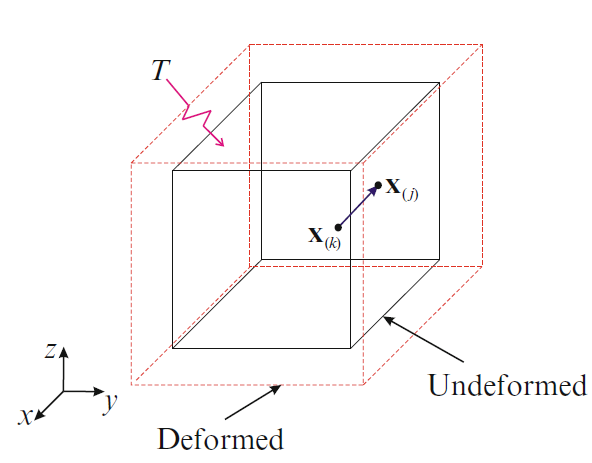
\includegraphics[width=0.5\linewidth]{./fig2.png}
  \caption{\label{fig:2}
  A three-dimensional body subjected to isotropic expansion. Image from \blue{\cite{madenci2014peridynamic}}.
}
\end{figure}

In this case we have
\begin{eqnarray}
  \epsilon_{xx(k)} =  \epsilon_{yy(k)} = \epsilon_{zz(k)} = \zeta\\
  \epsilon_{xy(k)} =  \epsilon_{xz(k)} = \epsilon_{yz(k)} = 0
\end{eqnarray}
Using representations from classical continuum mechanics, we could explicitly get the values of strain energy density $W_{(k)}$ and dilatation $\theta_{(k)}$:
\begin{equation}
W_{(k)} = \frac{9}{2}\kappa\zeta^2\\
\label{eq:33}
\end{equation}
\begin{equation}
\theta_{(k)} = \epsilon_{xx(k)}+\epsilon_{yy(k)}+\epsilon_{zz(k)} = 3\zeta.
\label{eq:34}
\end{equation}
The deformed relative position can be written in terms of relative position in reference(undeformed) space as:
\begin{equation}
|\mb{y}_{(j)} - \mb{y}_{(k)}| = (1+\zeta)|\mb{x}_{(j)} - \mb{x}_{(k)}|.
\label{eq:35}
\end{equation}
We also define $\bm{\xi} = \mb{x}_{(j)} - \mb{x}_{(k)}$, $\xi = |\bm{\xi}|$.
Calculation of $W_{(k)}$ and $\theta_{(k)}$ in peridynamics requires an integral over a sphere of radius $\delta$:
\begin{equation}
\begin{aligned}
W_{(k)} =& a\theta_{(k)}^2
           +b\sum_{j=1}^{N}w_{(k)(j)}(s_{(k)(j)}|\mb{x}_{(j)}-\mb{x}_{(k)}|V_{(j)})\cdot(s_{(k)(j)}|\mb{x}_{(j)}-\mb{x}_{(k)}|V_{(j)})\\
        =& a\theta_{(k)}^2
           +b\int_0^\delta\int_0^{2\pi}\int_0^{\pi}\frac{\delta}{\xi}\left[(1+\zeta)\xi-\xi\right]^2\xi^2\sin(\phi)d\phi d\theta d\xi\\
        =& 9a\zeta^2+\pi b\delta^5\zeta^2
\end{aligned}
\label{eq:36}
\end{equation}
and
\begin{equation}
\begin{aligned}
\theta_{(k)} =& d\sum_{j=1}^{N}w_{(k)(j)}s_{(k)(j)}\frac{\mb{y}_{(j)} - \mb{y}_{(k)}}{|\mb{y}_{(j)} - \mb{y}_{(k)}|}\cdot(\mb{x}_{(j)}-\mb{x}_{(k)})V_{(j)}\\
        =& d\int_0^\delta\int_0^{2\pi}\int_0^{\pi}\frac{\delta}{\xi}\left[(1+\zeta)\xi-\xi\right](\frac{\bm{\xi}}{\xi}\cdot\frac{\bm{\xi}}{\xi})\xi^2\sin(\phi)d\phi d\theta d\xi\\
        =& \frac{4\pi d\delta^4}{3}\zeta,
\end{aligned}
\label{eq:37}
\end{equation}
where $(\xi,\theta,\phi)$ are spherical coordinates. Comparing Equation \blue{\ref{eq:36}}, \blue{\ref{eq:37}} with Equation \blue{\ref{eq:33}}, \blue{\ref{eq:34}} leads to the consequent results:
\begin{equation}
9a + \pi b\delta^5 = \frac{9}{2}\kappa
\label{eq:38}
\end{equation}
\begin{equation}
d = \frac{9}{4\pi\delta^4}.
\label{eq:39}
\end{equation}

\noindent{\textbf{Case 2: simple shear}}

Figure \blue{\ref{fig:3}} illustrates an example of simple shear.
\begin{figure}[h]
\center
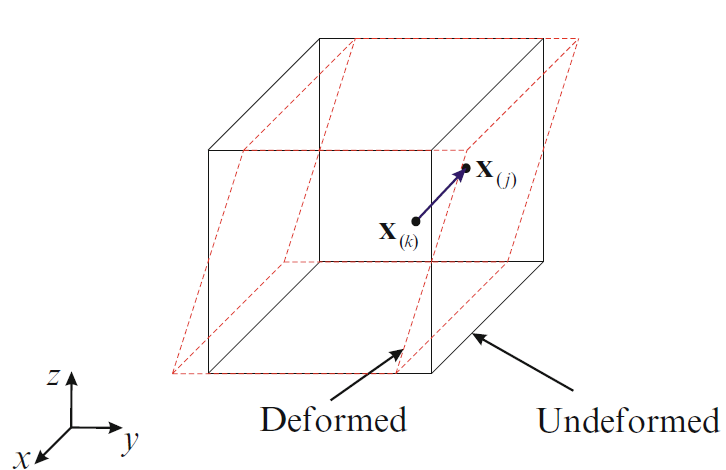
\includegraphics[width=0.5\textwidth]{fig3.png}
\caption{A three dimensional body subject to simple shear. Image from \blue{\cite{madenci2014peridynamic}}.
\label{fig:3}
}
\end{figure}

In this case, we have
\begin{equation}
\gamma_{xy(k)} = \zeta
\label{eq:40}
\end{equation}
\begin{equation}
\sigma_{xx(k)} = \sigma_{yy(k)} = \sigma_{zz(k)} = \gamma_{xz(k)} =\gamma_{yz(k)} = 0
\label{eq:41}
\end{equation}
and
\begin{equation}
|\mb{y}_{(j)} - \mb{y}_{(k)}| = (1+\frac{\zeta\sin(2\phi)\sin(\theta)}{2})|\mb{x}_{(j)} - \mb{x}_{(k)}|.
\label{eq:42}
\end{equation}

Strain energy density $W_{(k)}$ and dilatation $\theta_{(k)}$ within realm of classical continuum mechanics become:
\begin{equation}
W_{(k)} = \frac{1}{2}\mu\zeta^2\\
\label{eq:43}
\end{equation}
\begin{equation}
\theta_{(k)} = 0.
\label{eq:44}
\end{equation}

We can also calculate the strain energy density from
\begin{equation}
\begin{aligned}
W_{(k)} =& b\sum_{j=1}^{N}w_{(k)(j)}(s_{(k)(j)}|\mb{x}_{(j)}-\mb{x}_{(k)}|V_{(j)})\cdot(s_{(k)(j)}|\mb{x}_{(j)}-\mb{x}_{(k)}|V_{(j)})\\
        =& b\int_0^\delta\int_0^{2\pi}\int_0^{\pi}\frac{\delta}{\xi}\left[(1+\frac{\zeta\sin(2\phi)\sin(\theta)}{2})\xi-\xi\right]^2\xi^2\sin(\phi)d\phi d\theta d\xi\\
        =& \frac{b\pi\delta^5\zeta^2}{15}.
\end{aligned}
\label{eq:45}
\end{equation}
Equating Equation \blue{\ref{eq:43}} and \blue{\ref{eq:45}} yields:
\begin{equation}
b = \frac{15\mu}{2\pi\delta^5}.
\label{eq:46}
\end{equation}
Substituting Equation \blue{\ref{eq:46}} into Equation \blue{\ref{eq:38}} results in the determination of parameter $a$:
\begin{equation}
a = \frac{1}{2}(\kappa - \frac{5\mu}{3}).
\label{eq:47}
\end{equation}

\subsection{An intuitive comprehension}

We have derived the explicit form of the internal force density in previous sections (See Equation \blue{\ref{eq:29}},\blue{\ref{eq:30},\blue{\ref{eq:39}},\blue{\ref{eq:46}},\blue{\ref{eq:47}}}). Now we present an intuitive comprehension of the model, which leads to the final form of the force density that appears in the paper.

The force density is separated into the $dilatational$ part and the $deviatoric$ part. We start by dividing $a$ into two parts:
\begin{equation}
a = a_1 + a_2 \qquad \mathrm{with}\quad a_1 = \frac{1}{2}\kappa \quad a_2 = -\frac{5\mu}{6}.
\label{eq:48}
\end{equation}
Then $A$ is recast to
\begin{equation}
\begin{aligned}
A =4w_{(k)(j)}\left\{a_1d\frac{\mb{y}_{(j)}-\mb{y}_{(k)}}{|\mb{y}_{(j)}-\mb{y}_{(k)}|}\cdot\frac{\mb{x}_{(j)}-\mb{x}_{(k)}}{|\mb{x}_{(j)}-\mb{x}_{(k)}|}\theta_{(k)}
   +b\left(e_{(j)(k)} + \frac{a_2d}{b}\frac{\mb{y}_{(j)}-\mb{y}_{(k)}}{|\mb{y}_{(j)}-\mb{y}_{(k)}|}\cdot\frac{\mb{x}_{(j)}-\mb{x}_{(k)}}{|\mb{x}_{(j)}-\mb{x}_{(k)}|}\theta_{(k)}\right) \right\}
\end{aligned}
\label{eq:49}
\end{equation}
with
\begin{equation}
e_{(j)(k)} = (|\mb{y}_{(j)} - \mb{y}_{(k)}| - |\mb{x}_{(j)} - \mb{x}_{(k)}|)
\label{eq:50}
\end{equation}
defined as the extension between two material points. Note that the first term in brace is only associated with the bulk modulus $\kappa$ and the second term in brace is only related to the shear modulus $\mu$.
It shows that we have decoupled the dilatational and the deviatoric components of deformation.
Extension $e_{(j)(k)}$ amounts to the cauchy strain in classical mechanics, and we would define the deviatoric component of extension through:
\begin{equation}
\begin{aligned}
e^d_{(j)(k)} \equiv& e_{(j)(k)} + \frac{a_2d}{b}\frac{\mb{y}_{(j)}-\mb{y}_{(k)}}{|\mb{y}_{(j)}-\mb{y}_{(k)}|}\cdot\frac{\mb{x}_{(j)}-\mb{x}_{(k)}}{|\mb{x}_{(j)}-\mb{x}_{(k)}|}\theta_{(k)}\\
                  =& e_{(j)(k)} - \frac{\delta}{4}\frac{\mb{y}_{(j)}-\mb{y}_{(k)}}{|\mb{y}_{(j)}-\mb{y}_{(k)}|}\cdot\frac{\mb{x}_{(j)}-\mb{x}_{(k)}}{|\mb{x}_{(j)}-\mb{x}_{(k)}|}\theta_{(k)}.
\end{aligned}
\label{eq:51}
\end{equation}

Finally, we could rewrite $A$ as a more intuitive form
\begin{equation}
A = A_{dil} + A_{dev}
\end{equation}
with
\begin{equation}
A_{dil} = 4w_{(k)(j)} a\frac{\mb{y}_{(j)}-\mb{y}_{(k)}}{|\mb{y}_{(j)}-\mb{y}_{(k)}|}\cdot\frac{\mb{x}_{(j)}-\mb{x}_{(k)}}{|\mb{x}_{(j)}-\mb{x}_{(k)}|}\theta_{(k)}
\end{equation}
\begin{equation}
A_{dev} = 4w_{(k)(j)} b e^d_{(j)(k)},
\end{equation}
where we redefine $a$ as
\begin{equation}
a = a_2d = \frac{9\kappa}{8\pi\delta^4}.
\end{equation}
The above reformulation produces the exact elastic constitutive model used in our paper.


\bibliographystyle{eg-alpha}
\bibliography{../references}

\end{document}
